%!TEX root = .../tfg_im.tex

\chapter{Desarrollo}

\section{Descripción}

\subsection{Funciones del sistema}

\displayquote{``La aplicación que se va a desarrollar tiene como objetivo recoger información de las diferentes redes sociales, almacenarlos en una base de datos y mostrarlos en nuestro sitio web. Esos datos almacenados,son una fuente de información fiable que nos permite conocer que se esta concinando en el mundo en este momento. Para ello se deberá tener en cuenta la gestión de:''}


\vspace{5 mm}

\begin{itemize}

\item Control de Acceso: En la aplicación existirán 3 tipos de roles:

\begin{itemize}
\item Administrador: Tendrá el control de gestionar la información proveniente de las API's.El Filtrado de los datos o la frecuencia con la que realiza las peticiones la aplicación con las API's.
También podrá gestionar el contenido del sistema
\item Colaborador: Podrá publicar contenido en la aplicación.
\item Usuario no registrado: Tendrá acceso a la visualización de los datos de la aplicación. 
\end{itemize}

\end{itemize}

\section{Análisis}

Para el desarrollo de la aplicación se lleva a cabo previamente un análisis de las diferentes herramientas utilizadas.

\subsection{Twitter}

Twitter es la red social de \textquote{microblogging} más conocida actualmente. Esta red social tiene mas de 500 millones de usuarios, generando un número aproximado de 65 millones de tweets al dia. Es por ello que se optó por Twitter, ya que es una gran fuente de información.

\vspace{5 mm}

Toda la información proveniente de Twitter es guardada en la base de datos de la aplicación. Para obtener la información, Twitter porporciona una REST API que proporciona a los desarrolladores un acceso a la lectura y escritura de toda la información disponible en la red social.

\vspace{5 mm}

\textbf{Twitter API}

\vspace{5 mm}

\begin{figure}
\begin{center}
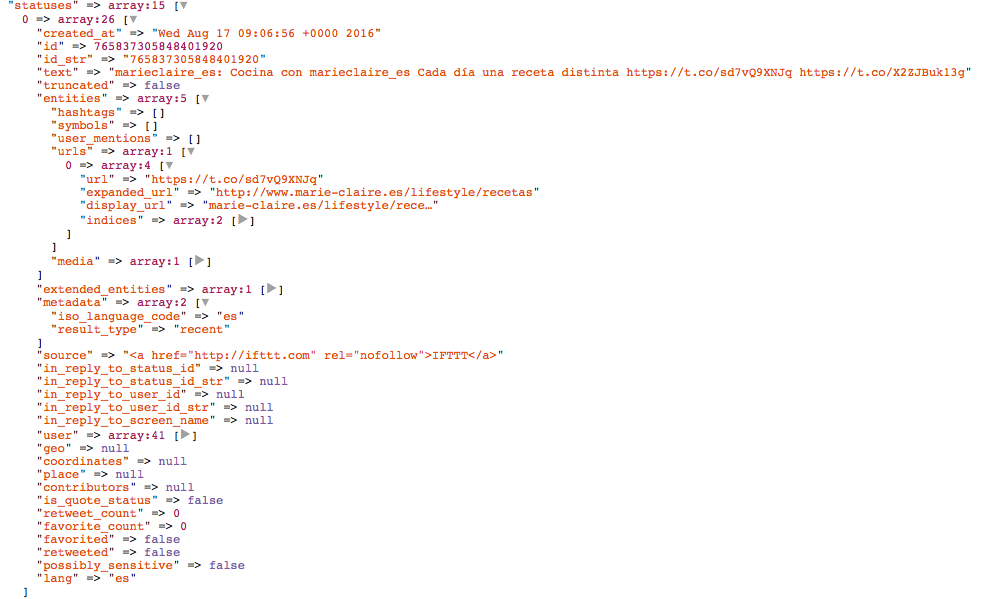
\includegraphics[width=1.0\textwidth]{imagenes/estructura-tweet.png}
\caption{Estrucutra de un tweet}
\label{tweet}
\end{center}
\end{figure}

La REST API de Twitter nos proporciona los datos en formato JSON listos para ser procesados. Un Tweet, contiene una estructura(ver figura \ref{tweet}) elaborada con toda la información relacionada. La estructura de un Tweet consta de los siguientes elementos:

\begin{itemize}

\item \textbf{created\_at}: Fecha de creación del Tweet, contiene el dia, mes, hora, zona horaria y año cuando se ha creado el Tweet.
\item \textbf{id}: Identificador único del Tweet
\item \textbf{id\_str}: El identificador del Tweet en formato de cadena de texto. Este campo esta creado para ciertos lenguajes que no soportan enteros mayores de 53 bits, como es el caso de Javascript.
\item \textbf{text}: Contiene la información del Tweet(máximo de 140 caracteres).
\item \textbf{truncated}: Booleano que especifíca si el valor del campo text está cortado. El texto truncado terminará con los tres puntos suspensivos.
\item \textbf{entities}: Proporciona metadatos asociados al contenido del tweet. Entities es un objeto que contiene los siguientes elementos:

\begin{itemize}

\item \textbf{hashtags}: Representa un array con los hashtags parseados en el contenido del tweet. Cada hastag contiene un campo de texto con el contenido del hashtag y un array de enteros indicando la posicion inicial y final que ocupa en el Tweet.

\item \textbf{media}: Array de objetos que representa el contenido multimedia subido en el Tweet. Este array contiene la url para mostrar a los clientes(display\_url). Una versión expandida de la url(expanded\_url). El id del fichero y el id en formato de cadena de texto(id\_str). Un array con los indíces de la posiciones inicial y final de la url en el texto. Una url apuntando directamente al fichero subido(media\_url) y una url para páginas https(media\_url\_https). Un objeto con los tamaños disponibles para el fichero(sizes).Para aquellos tweets que tiene contenido multimedia asociado a otros tweets, se guarda un identificador que apunta al Tweet con el contenido original(source\_status\_id). El tipo de fichero(type) y la url incrustada en el contenido del Tweet(url).

\item  \textbf{url}: Contiene un array de objetos que representan las urls incluidas en el texto. Contiene la url de visualización, la url expandida y los indices donde se encuentra la url.

\item \textbf{user\_mentions}: Representa otros usuarios de twitter mencionados en el texto del tweet. Este array tiene el id del usuario mencionado, el id en string, los indices y el nombre(name).

\end{itemize}


\item \textbf{metadata}: Array de objetos metadatos asociados al tweet.

\begin{itemize}

\item \textbf{iso\_language\_code}: Codificación iso del lenguaje del tweet.

\item \textbf{result\_type}: Especifica el tipo de resultado de tweet que quieres recibir. El valor por defecto es recent que devuelve un resultado con los tweets más recientes. También están los valores popular que devuelve los tweets más populares y mixed que incluye ambos tipos mencionados anteriormente.

\end{itemize}


\item \textbf{in\_reply\_to\_status\_id}: Si el tweet es una respuesta de otro tweet, este campo tendrá el id del tweet orginal.

\item \textbf{in\_reply\_to\_user\_id}: Contendrá el id del usuario del Tweet original.

\item \textbf{user}: Contiene un array de objetos con toda la información relativa a el usuario que ha publicado el Tweet.

\begin{itemize}

\item \textbf{id}: id del usuario que pública el Tweet.

\item \textbf{name}: Nombre del usuario.

\item \textbf{location}: Cadena de caracteres con el sitio geaográfico al que pertenece el usuario.

\item \textbf{description}: Pequeño resumen descriptivo sobre el usuario.

\item \textbf{url}: Url proporcionada por el usuario asociada con su perfil.

\item \textbf{followers\_count}: Número de seguidores que tiene el usuario.

\item \textbf{friends\_count}: Número de personas a las que sigue el usuario.

\item \textbf{protected}: Indica si la cuenta del usuario esta protegida, es decir que sus Tweets solo pueden ser vistos con el consentimiento del usuario.

\item \textbf{geo\_enabled}: Indica si el usuario a activado la posibilidad de geoetiquetar sus Tweets, es decir, agregar información geográfica en los metadatos del tweet.


\end{itemize}

\item \textbf{coordinates}: Representa la posicion geográfica del Tweet. El array de coordenadas esta en geoJSON, donde la longitud es el primer elemento del array y la latitud el segundo.

\item \textbf{place}: Cuando el Tweet esta asociado a un lugar, pero no necesariamente es orginado de ahí.

\item \textbf{retweet\_count}: Numero de veces que el Tweet ha sido retweeteado.

\item \textbf{lang}: Idioma en el que esta escrito el Tweet. 

\end{itemize}

\vspace{5 mm}

Con el análisis de la estructura de un Tweet realizado, se procede a buscar información en Twitter sobre datos relevantes para la aplicación. Para encontrar los datos relevantes que se ajusten a los requisitos para la aplicación, la API de Twitter proporciona unas opciones de búsqueda que permiten buscar los Tweets por palabras clave, idioma, localización y número.

\vspace{5 mm}

Para el caso de Njoycooking, se pretendía inicialmente buscar Tweets en español de la zona de la península Ibérica que tuvieran la palabra receta, cocina o comida en el Tweet. Para ello Twitter proporciona los siguientes parametros:

\begin{itemize}

\item \textbf{q}: Parámetro para realizar un consulta de búsqueda por palabras.

\item \textbf{geocode}: Parámetro que permite encontrar Tweets de usuarios localizados en un radio alrededor de un punto central proporcionado en latitud/longitud. Por ejemplo para buscar Tweets de la peninsula establecemos el centro en Madrid que en coordenadas lat/long es (39.8952506,-3.46863775058), y le decimos el radio de alcance, aproximadamente unos  500km.

\item \textbf{lang}: Parámetro que restringe la búsqueda de Tweets al idioma dado. Si solo utilizaramos el parámetro geocode twitter también nos sacaría resultados de Tweets en portugues, para ello se añade este parámetro indicandole que busque por el idioma español(es).

\item \textbf{count}: Parámetro que sirve para definir el número de Tweets a devolver por consulta. Por defecto son 15 y se puede buscar hasta un máximo de 100.


\item \textbf{until}: Devuelve los Tweets creados antes de la fecha dada. Este parámetro no tiene mucho sentido que se utilize, ya que lo que se pretende es buscar los últimos Tweets en tiempo real y no buscar por una fecha determinada.

\item \textbf{result\_type}: Parámetro para especificar el tipo de resultado de búsqueda. Los tipos son mixed,recent,popular. Para la aplicación interesa el tipo de resultados recent, ya que nos devuelve los Tweets más recientes. 

\end{itemize}


\subsection{Google Maps}



\section{Especificación de Requisitos}

Para este apartado se ha seguido el estándar IEEE 830 de especificación de requisitos.

\subsection{Requisitos funcionales}

Para ordenar los requisitos funcionales, se ha considerado que la forma más adecuada es por tipo de rol y relevancia. Los identificadores de los requisitos que pertenezcan al rol de administrador empezarán por A, los que pertenezcan al rol de usuario empezarán por U, los que pertenezcan al sistema empezarán por S. Para ordenar por relevancia, se especificán tres casos: Los requisitos que sean funcionalidades básicas de la aplicación empezarán por FB, los requisitos que sean funcionalidades secundarias empezarán FS.

\vspace{5 mm}


%Requisito 1 usuario
\begin{table}[h!]
\centering
\begin{tabular}{|p{3cm}|p{10cm}|}
\hline
Identificador & FB-U-01 \\ \hline
Actor involucrado & Usuario \\ \hline
Nombre & Ver listado de entradas \\ \hline
Descripción & Desde la página de blog o un buscador se podrá acceder a ver un listado de las entradas del blog. Cada elemento del listado contendrá una foto de la entrada, un titulo y un resumen \\ \hline
Requisitos lógicos & Podrán existir una serie de datos generados por usuarios,como comentarios. \\ \hline
\end{tabular}
\end{table}


%Requisito 2 usuario
\begin{table}[h!]
\centering
\begin{tabular}{|p{3cm}|p{10cm}|}
\hline
Identificador & FB-U-02 \\ \hline
Actor involucrado & Usuario \\ \hline
Nombre & Ver detalle de entrada \\ \hline
Descripción & En el detalle de la entrada,  \\ \hline
Requisitos lógicos & La información estará normalizada, existiendo una serie de datos comunes a todas las entradas, pero podrán existir ciertos datos adicionales según el tipo de entrada. También podrán existir una serie de datos generados por usuarios, como valoraciones y comentarios. \\ \hline
\end{tabular}
\end{table}


%Requisito 3 usuario
\begin{table}[h!]
\centering
\begin{tabular}{|p{3cm}|p{10cm}|}
\hline
Identificador & FB-U-03 \\ \hline
Actor involucrado & Usuario \\ \hline
Nombre & Comentar Entrada\\ \hline
Descripción & En el detalle de la entrada,  \\ \hline
Requisitos lógicos & La información estará normalizada, existiendo una serie de datos comunes a todas las entradas, pero podrán existir ciertos datos adicionales según el tipo de entrada. También podrán existir una serie de datos generados por usuarios, como valoraciones y comentarios. \\ \hline
\end{tabular}
\end{table}

%Requisito 4 usuario
\begin{table}[h!]
\centering
\begin{tabular}{|p{3cm}|p{10cm}|}
\hline
Identificador & FB-U-04 \\ \hline
Actor involucrado & Usuario \\ \hline
Nombre & Ver listado de tweets\\ \hline
Descripción & En el mapa de la aplicación se geoposicionarán los tweets  \\ \hline
Requisitos lógicos & Los tweets \\ \hline
\end{tabular}
\end{table}


%Requisito 5 usuario
\begin{table}[h!]
\centering
\begin{tabular}{|p{3cm}|p{10cm}|}
\hline
Identificador & FB-U-05 \\ \hline
Actor involucrado & Usuario \\ \hline
Nombre & Filtrar listado de tweets\\ \hline
Descripción & En el detalle de la entrada,  \\ \hline
Requisitos lógicos & La información estará normalizada, existiendo una serie de datos comunes a todas las entradas, pero podrán existir ciertos datos adicionales según el tipo de entrada. También podrán existir una serie de datos generados por usuarios, como valoraciones y comentarios. \\ \hline
\end{tabular}
\end{table}

%Requisito 6 usuario
\begin{table}[h!]
\centering
\begin{tabular}{|p{3cm}|p{10cm}|}
\hline
Identificador & FB-U-06 \\ \hline
Actor involucrado & Usuario \\ \hline
Nombre & Login\\ \hline
Descripción & El usuario podrá loguearse en la aplicación como colaborador o administrador mediante un formulario de registro.  \\ \hline
Requisitos lógicos & Para loguearse será necesario introducir los campos de usuario y contraseña en el formulario.\\ \hline
\end{tabular}
\end{table}

%Requisito 1 admin
\begin{table}[h!]
\centering
\begin{tabular}{|p{3cm}|p{10cm}|}
\hline
Identificador & FB-A-01 \\ \hline
Actor involucrado & Administrador \\ \hline
Nombre & Ver listado de admin de entradas del blog\\ \hline
Descripción & En la sección de ver entradas, el administrador tendrá la opción de ver un listado de las entradas disponibles en la aplicación. En el caso de que quiera editar una entrada el usuario deberá ir al detalle. \\ \hline

\end{tabular}
\end{table}

%Requisito 2 admin
\begin{table}[h!]
\centering
\begin{tabular}{|p{3cm}|p{10cm}|}
\hline
Identificador & FB-A-02 \\ \hline
Actor involucrado & Administrador \\ \hline
Nombre & Gestionar una entrada de blog\\ \hline
Descripción & En el detalle de la entrada, el administrador podrá gestionar el contenido de la entrada  \\ \hline
Requisitos lógicos & La gestión del contenido implica la modificación de los campos de la entrada y el borrado. \\ \hline
\end{tabular}
\end{table}

%Requisito 3 admin
\begin{table}[h!]
\centering
\begin{tabular}{|p{3cm}|p{10cm}|}
\hline
Identificador & FB-A-03 \\ \hline
Actor involucrado & Administrador \\ \hline
Nombre & Moderar comentarios\\ \hline
Descripción & En el detalle de la entrada, se mostrarán los comentarios asociados a la entrada que el administrador podrá moderar si sobrepasan las normas de comportamiento. \\ \hline
Requisitos lógicos & La información estará normalizada, existiendo una serie de datos comunes a todas las entradas, pero podrán existir ciertos datos adicionales según el tipo de entrada. También podrán existir una serie de datos generados por usuarios, como valoraciones y comentarios. \\ \hline
\end{tabular}
\end{table}

 %Requisito 4 admin
\begin{table}[h!]
\centering
\begin{tabular}{|p{3cm}|p{10cm}|}
\hline
Identificador & FB-A-04 \\ \hline
Actor involucrado & Administrador \\ \hline
Nombre & Moderar comentarios\\ \hline
Descripción & En el detalle de la entrada, se mostrarán los comentarios asociados a la entrada que el administrador podrá moderar si sobrepasan las normas de comportamiento. \\ \hline
Requisitos lógicos & La información estará normalizada, existiendo una serie de datos comunes a todas las entradas, pero podrán existir ciertos datos adicionales según el tipo de entrada. También podrán existir una serie de datos generados por usuarios, como valoraciones y comentarios. \\ \hline
\end{tabular}
\end{table}


\section{Casos de Uso}

\begin{landscape}
\begin{figure}
\begin{center}
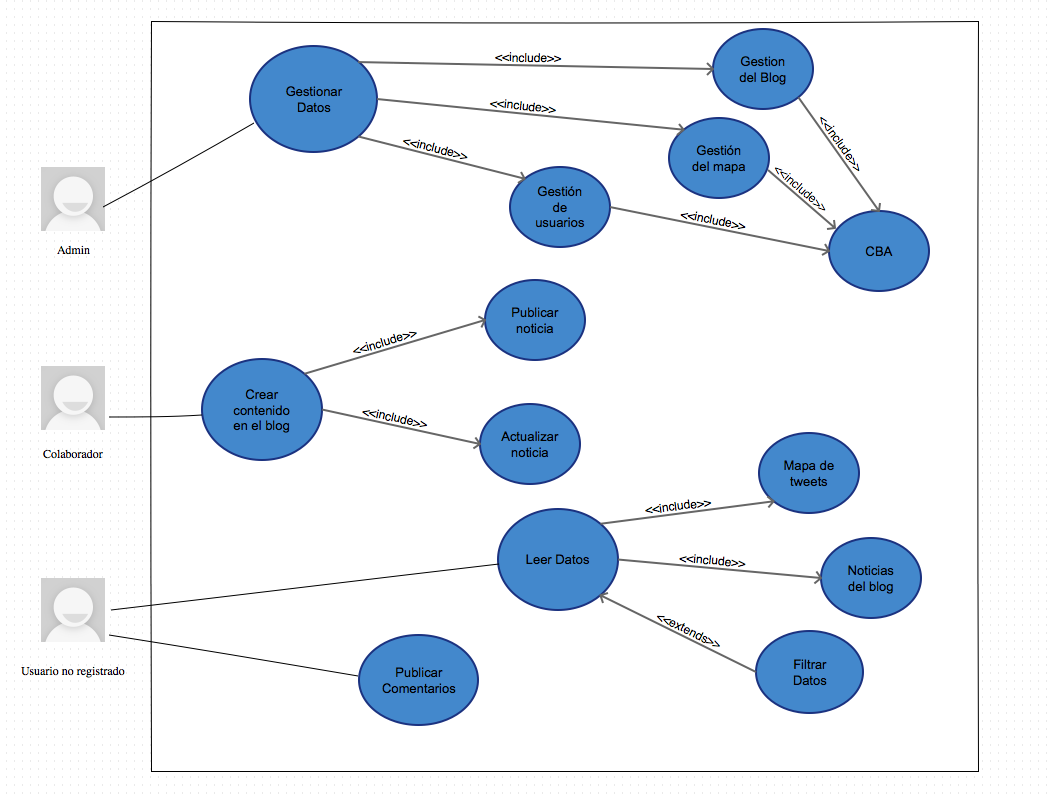
\includegraphics[width=16cm]{imagenes/casos-de-uso.png}
\caption{Casos de uso}
\label{casos_uso}
\end{center}
\end{figure}
\end{landscape}

Para mostrar las actividades se utilizará una representación mediante casos de uso. Los casos de uso se han segmentado para cada rol de la aplicación. En la figura \ref{casos_uso}  se representan los casos de uso para cada rol que se explicarán a continuación:

\vspace{5 mm}

El \textbf{usuario no registrado}, es el rol por defecto en la aplicación cuando el usuario no tiene ninguna acreditación en la web y carece de permisos. El usuario no registrado podrá solicitar los datos de la aplicación para visualizar el contenido. Por ejemplo podrá solicitar los datos del mapa de tweets o del blog. Tambíen podrá filtrar la información de los datos solicitados, por palabras clave o categorías. Este usuario podrá también publicar comentarios en el blog.

\vspace{5 mm}

El \textbf{colaborador}, este rol, además de poder realizar las mismas funciones que el usuario no registrado, tiene unos permisos añadidos. Este usuario tiene la función extra de publicar contenido en el blog. Un usuario colaborador, podrá crear noticias que luego aparecerán en el blog. Podrá actualizar las noticias, pero únicamente aquellas que hayan sido creadas por él. No tendrá permisos para borrar contenido del blog.

\vspace{5 mm}

Por último esta el \textbf{administrador}, el rol de administrador, es el de superusuario, ya que posee todos los permisos. El administrador es el encargado de gestionar todo el contenido de la web. Dentro del contenido se encuentran los tres principales modelos de datos. El primer modelo de datos son los \textquote{Tweets}, el administrador se encargará de gestionar la frecuencia con la que se actualiza el mapa de tweets, para tener representada la información actualizada. Otra función será modificar la recolección de tweets en base a una palabra clave, que el administrador introducirá manualmente. El siguiente modelo son las noticias, el administrador podrá generar contenido en el blog, creando o borrando cualquier tipo de contenido, tanto propio como de un colaborador. El administrador también podrá moderar los comentarios de las entradas del blog. Por último el último el último modelo de datos serían los usuarios. El administrador gestionará los datos de los usuarios de la aplicación, siendo el encargado tanto de dar de alta a los colaboradores generando un usuario y contraseña como darlos de baja. Toda la gestión del contenido implica crear,borrar o actualizar información de forma que se ha representado mediante un caso de uso: CBA.


\section{Diseño de Arquitectura}

\subsection{Arquitectura MVC}

\begin{figure}
\begin{center}
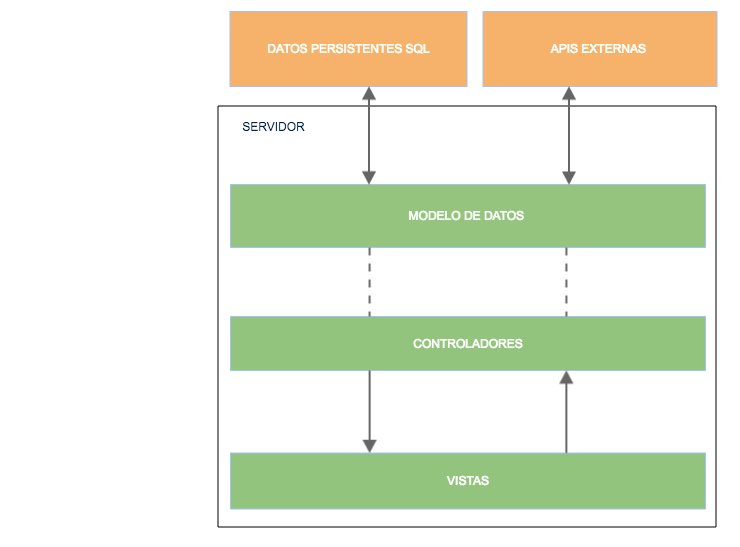
\includegraphics[width=1.0\textwidth]{imagenes/arquitectura.png}
\caption{Arquitectura de la aplicación}
\label{arquitectura}
\end{center}
\end{figure}



La rama de la ingenieria del software se preocupa por crear productos robustos y de calidad. Una de las principales soluciones para conseguir esos objetivos, es la arquitectura basada en capas, que separa el código en función de sus responsabilidades.Una de las arquitecturas más populares basada en capas para el desarrollo de aplicaciones web, es la arquitectura MVC(Modelo-Vista-Controlador). En la figura \ref{arquitectura} se muestra un esquema de la arquitectura de la aplicación.

\begin{itemize}

\item \textbf{Modelo de datos}: Capa que trabaja con los datos, contiene mecanismos para acceder a la información. A través del modelo accederemos a la base de datos donde,estará la información almacenada. Mediante los modelos también se accederá a los datos de servicios externos que posteriormente se guradarán en la base de datos.

\item \textbf{Controladores}: Responde generalmente a acciones del usuario, e invoca esas peticiones al modelo. También responde al envío de datos a la vista. Los controladores son el núcleo de la aplicación, ya que es aquí donde se procesan todos lo datos antes de ser enviados a la vista. Un controlador consta de varios métodos, cada método se corresponde con una vista y hace uso de las diferentes clases de la capa de modelos de datos. 

\item \textbf{Vistas}: Es la capa encargada de presentar la información de nuestra página. Los datos provenientes del controlador se presentan en las vistas para que luego ser renderizada por el navegador.

\end{itemize}

 EL flujo de la información en la aplicación sería el siguiente: El usuario accederá a una ruta a través del navegador. Cada ruta de la aplicación se corresponde con una vista, que a su vez esta asociada a un controlador. En el controlador correspondiente se llama a las distintas clases de los modelos. Los modelos conectan con la base de datos, esta le devuelve la información, y es recibida y procesada por los controladores que la envían a la vista para que se visualize en el navegador. 


%El diagrama de la figura \ref{logo_mvc}

\vspace{5 mm}

Crear una aplicación web basada en la arquitectura MVC nos ofrece ciertas ventajas. Por ejemplo, se puede dividir la lógica del negocio del diseño del sistema, haciendo el proyecto más escalable. Otra ventaja, es la existencia  de muchos frameworks basados en MVC como Laravel o Yii Framework, que permiten facilitar el trabajo de los desarrolladores. La implementación de URLs amigables, el control del uso de la memoria caché o el control de los recursos del servidor son tres de las principales ventajas de usar un framework MVC.


\section{Modelo de Datos}

Como se ha comentado en el apartado anterior, el modelo de datos elegido para almacenar la información es el modelo relacional MySQL. El modelo relacional se fundamenta en el uso de relaciones, estas relaciones se pueden considerar como un conjunto de datos. Para mostrar una forma más visual esas relaciones se conceptualizan en forma de tablas, que estan formadas por registros y campos. En la figura \ref{tablas_bd} se representa mediante un modelo entidad-relacion los conjuntos de datos para la aplicación. Todas las tablas continene un campo Id que es el identificador de cada tabla(clave primaria) y tienen la clausula de auto-incremento por lo que cada vez que se agregue una fila, MySQL nos generará otro identificador incrementandolo en 1 valor.


\begin{figure}
\begin{center}
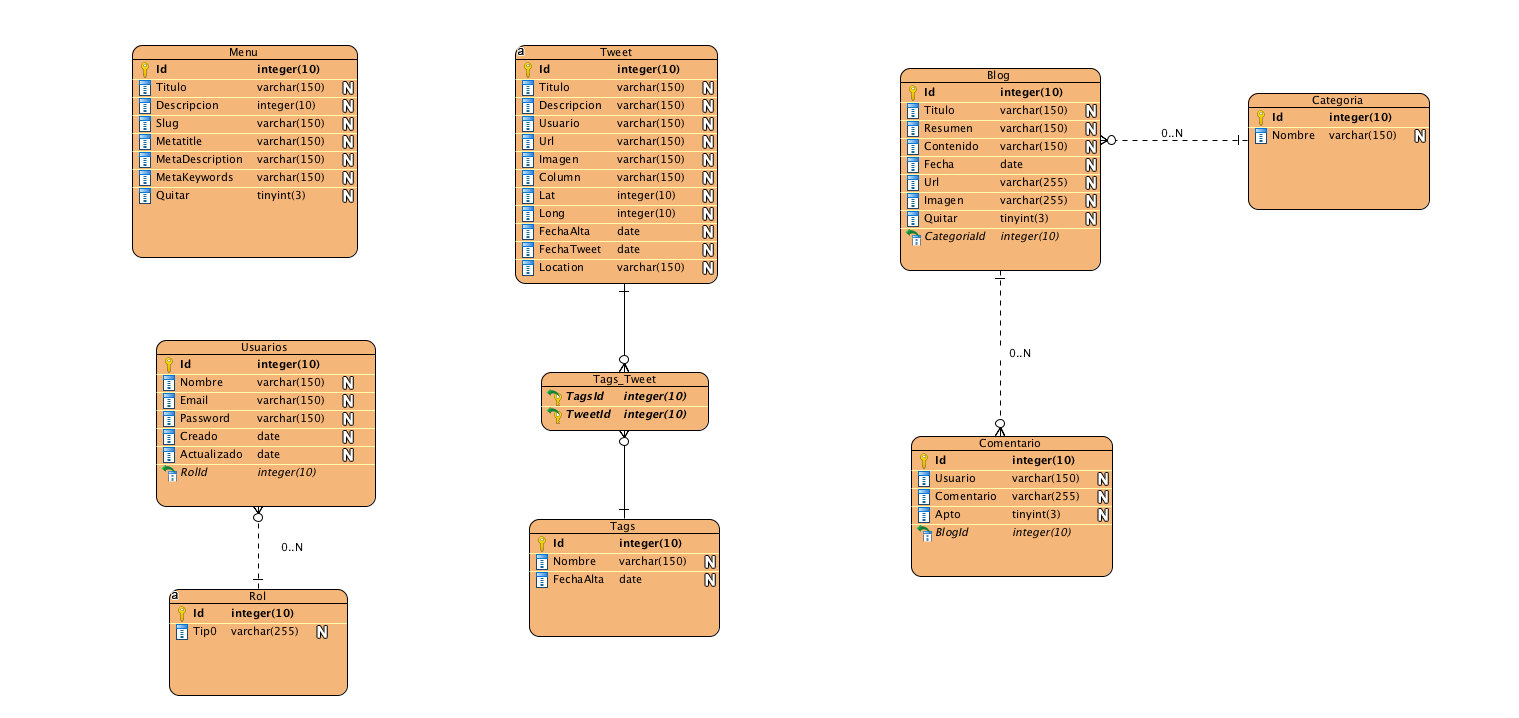
\includegraphics[width=1.0\textwidth]{imagenes/E-R.png}
\caption{Conjunto de tablas}
\label{tablas_bd}
\end{center}
\end{figure}

\begin{figure}
\begin{center}
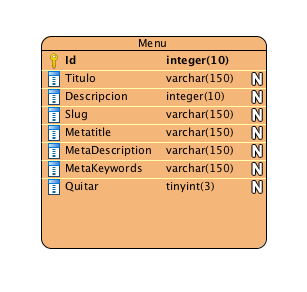
\includegraphics[scale=0.7]{imagenes/menu.png}
\caption{Tabla del menú}
\label{menu_bd}
\end{center}
\end{figure}

\begin{figure}
\begin{center}
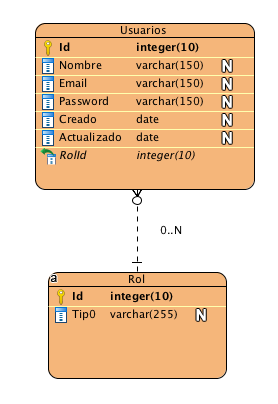
\includegraphics[scale=0.7]{imagenes/Usuarios.png}
\caption{}
\label{users_bd}
\end{center}
\end{figure}

\begin{figure}
\begin{center}
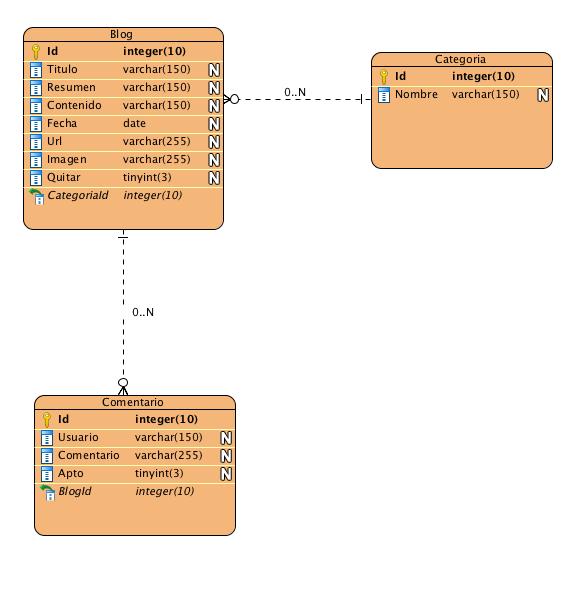
\includegraphics[scale=0.7]{imagenes/blog.png}
\caption{Tablas para el blog}
\label{blog_bd}
\end{center}
\end{figure}

\begin{figure}
\begin{center}
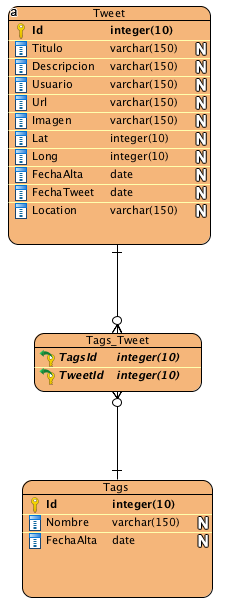
\includegraphics[scale=0.7]{imagenes/map.png}
\caption{Tablas para el mapa}
\label{map_bd}
\end{center}
\end{figure}


\vspace{5 mm}

La primera tabla, y más básica es la tabla de Menus, en ella encontramos todos los datos correspondientes al menu de navegación de la aplicación,esta tabla esta pensada para que el menú sea más dinamico y se pueda gestionar de forma más fácil sin modificar código. COmo se observa en la figura \ref{menu_bd}, la tabla de Menú se compone de los siguientes elementos:

\begin{itemize}

\item \textbf{Titulo}: Este es el titulo del menú, y el que aparecerá en la web en la navegación.
\item \textbf{Descripcion}: Campo para añadir texto introductorio, acerca de la sección.
\item \textbf{Slug}: El slug corresponde al trozo de la url que aparecerá para esa sección de la web en la aplicación.
\item \textbf{Campos de MetaAtributos}: MetaKeywords,MetaDescription,MetaTitle, los metas para cada sección del menú. Estos campos son importantes para un buen posicionamiento SEO.
\item \textbf{Quitar}: Campo de tipo tinyint, que nos permite dejar de mostrar un elemento del menú sin tener que borrar la fila. Por defecto el campo quitar esta a 0 y por tanto mostrará el elemento, en el caso de no se quiera visualizar, se cambia el valor a 1 y ese elemento ya no se muestra en el menu.

\end{itemize}

\vspace{5 mm}

En la figura \ref{users_bd}, se muestra la tabla de Usuarios y su relacion con los Roles de la aplicación. Se pretendía que un usuario tuviera un único rol y que un rol pudiera ser adoptado por muchos usuarios. Para representar esa relación se añade un clave ajena en la tabla usuarios generando una relacion uno a muchos y así permitiendonos cumplir las condiciones dictadas previamente.Para la tabla de Usuarios, se generan los siguientes campos:

\begin{itemize}

\item \textbf{Nombre}: Nombre del usuario, que se muestra en la web.
\item \textbf{Email}: Correo electrónico, del usuario. Tanto este campo como el nombre sirven de login para el usuario.
\item \textbf{Password}: Contraseña del usuario. En la base de datos se guarda un hash de la contraseña para mayor seguridad.
\item \textbf{Creado}: Campo de fecha con la creación del usuario.
\item \textbf{Actualizado}: Campo de fecha con la actualización del usuario.
\item \textbf{RolId}: Clave ajena a la tabla de Rol, contiene el Id del Rol.

\end{itemize}

\vspace{5 mm}

La tabla de Rol únicamente contiene el campo identificador y el tipo que hace referencia al nombre del rol.

\vspace{5 mm}

Para la página del Blog \ref{blog_bd} tenemos el esquema relacional con tres tablas: Blog,Categoría y Comentario. Cada fila de la tabla pertenece a una noticia del blog de la aplicación, cada noticia puede tener uno o más comentarios y ese comentario podrá aparecer solo en una noticia. Por tanto para cumplir esas condiciones se generan dos tablas(Blog y Comentario) con una relación uno a muchos. Las noticias pueden tener categorías, en el caso de la aplicación una noticía puede pertenecer a una categoría o ninguna, por tanto se añade una relación muchos a uno de la tabla Categoría a Blog. Las tuplas para la tabla de Blog son las siguientes:


\begin{itemize}

\item \textbf{Título}: Título de la noticia.
\item \textbf{Resumen}: Campo de texto para mostrar un resumen en el listado de noticias.
\item \textbf{Contenido}: Contenido de la noticia.
\item \textbf{Fecha}: Campo de Fecha con la creación de la noticia.
\item \textbf{Url}: Url amigable que aparece en la ruta de la noticia.
\item \textbf{Imagen}: Campo de texto para la imagen principal de la noticia.
\item \textbf{Quitar}: Campo quitar, para poder dejar de visualizar la noticia sin necesidad de borrarla de la base de datos.
\item \textbf{CategoríaId}: Clave ajena. Id de la categoría a la que pertenece la noticia.

\end{itemize}

\vspace{5 mm}

Tuplas para la tabla de comentarios:

\begin{itemize}

\item \textbf{Usuario}: Usuario que comenta la noticia.
\item \textbf{Comentario}: Campo de texto con el comentario sobre la noticia.
\item \textbf{Apto}: Campo para moderar el comentario y que sea valido para mostrar. Por defecto vale 1, no se muestra, cuando se cambia a cero se valida y se muestra.
\item \textbf{BlogId}: Clave ajena con el Id de la noticia al que pertence el comentario.


\end{itemize}

\vspace{5 mm}

Para el mapa de tweets se generan tres tablas(figura \ref{map_bd}). La principal es la tabla Tweet, donde se almacenan todos los tweets que se van a mostrar en el mapa. Los campos son los siguientes:


\begin{itemize}

\item \textbf{Título}: Título del tweet.
\item \textbf{Descripción}: Campo de texto que contiene el tweet.
\item \textbf{Usuario}: Usuario que ha escrito el tweet
\item \textbf{Url}: Enlace que se encuentra en el tweet y que te lleva a una página externa.
\item \textbf{Imagen}: Imagen del tweet.
\item \textbf{Lat}: Coordenada de latitud en el mapa.
\item \textbf{Long}: Coordenada de longitud en el mapa.
\item \textbf{FechaAlta}: Fecha de registro del tweet.
\item \textbf{FechaTweet}: Fecha de creación del tweet.
\item \textbf{Location}: Campo que guarda una localización.

\end{itemize}


\vspace{5 mm}


Para clasificar el contenido de los tweets, se crea la tabla Tags, que son los distintas clases en las que se pueden clasificar los tweets. Los campos para esta tabla son, el nombre de la etiqueta y la fecha de registro de la misma.

\vspace{5 mm}

Según como esta especificado, un tweet puede tener uno o más tags, y pueden pertenecer varios tweets a un tag. Por tanto es una relación muchos a muchos, para cumplir esta relación se crea una tabla adicional(Tag\_Tweets), que contiene los identificadores(es decir las claves primarias) de las dos tablas relacionadas(Tweet y Tag).









